% ============================================================
%  AI 图像检索项目实验报告
%  基于提供的深圳大学实验报告模板改写
% ============================================================

\documentclass[a4paper,12pt]{article}
\usepackage{fontspec}
\usepackage{xeCJK}
\setCJKmainfont{Noto Serif CJK SC}
\usepackage{geometry}
\geometry{left=1in, right=1in, top=1in, bottom=1in}
\usepackage{longtable}
\usepackage{graphicx}
\usepackage{fancyhdr}
\usepackage{tikz}
\usetikzlibrary{calc}
\usepackage{verbatim}
\usepackage{float}
\usepackage{subcaption}

\pagestyle{fancy}
\fancyhf{}
\fancyhead[L]{AI 图像检索项目实验报告}
\fancyhead[C]{}
\fancyhead[R]{}

\begin{document}

% 封面
\begin{titlepage}
    \centering
    \vspace*{1.5cm}
    \Huge{\textbf{AI 图像检索项目实验报告}}\\[1.2cm]
    \Large{课程名称:\underline{计算机视觉 / 深度学习实训}}\\[0.6cm]
    \Large{项目名称:\underline{ai_image_retrieval — 基于 DINOv2 的图像检索系统}}\\[0.6cm]
    \Large{学 \qquad 院:\underline{人工智能学院}}\\[0.6cm]
    \Large{专 \qquad 业:\underline{计算机科学与技术}}\\[0.6cm]
    \Large{指导教师:\underline{}}\\[0.6cm]
    \Large{报告人:\underline{(填写你的姓名)} \quad 学号:\underline{}}\\[0.6cm]
    \Large{实验时间:\underline{2025 年 — 2026 年}}\\[1.5cm]
    \vfill
    \Large{项目仓库:\underline{ai\_image\_retrieval}}
\end{titlepage}

\newpage

\section{实验目的}
本实验旨在实现一个端到端的图像检索系统,掌握以下能力:
\begin{enumerate}
  \item 使用预训练视觉表征(DINOv2)提取图像特征;
  \item 构建特征数据库并实现高效相似度搜索(基于 NumPy 实现);
  \item 将检索流程与简单的 Web/Django 项目结合,支持图片上传与检索展示;
  \item 评估检索效果并总结工程实现要点与改进方向。
\end{enumerate}

\section{项目概述}
本项目目录结构(摘要)包含特征提取、数据库构建与检索相关脚本,以及一个用于展示/部署的 Django 项目:
\begin{itemize}
  \item \textbf{特征与模型文件}:`vit-dinov2-base.npz`(DINOv2 权重),`dinov2_numpy.py`(基于 NumPy 的提取器实现)。
  \item \textbf{数据库文件}:`db_features.npy`, `db_paths.npy`, `db_captions.npy`, `db.sqlite3`(可直接加载检索用的特征/路径)。
  \item \textbf{构建脚本}:`build_database.py`, `build_database_from_csv.py` 用于从图片或 CSV 构建/更新特征库。
  \item \textbf{检索模块}:`search/utils/feature_extractor_numpy.py`, `search/utils/similarity_search_numpy.py` 实现特征抽取与相似度计算。
  \item \textbf{演示与工具}:`calc.py`, `debug.py` 等脚本用于快速试验与调试检索流程。
  \item \textbf{Web 前端}:`image_search/` 项目与 `search/` 应用,包含视图、模板和静态文件用于展示检索结果。
\end{itemize}

\section{方法与实现}
\subsection{特征提取}
系统使用 DINOv2 基于 ViT 的视觉表征。实现要点:
\begin{itemize}
  \item 使用 `dinov2_numpy.py` 或 `search/utils/feature_extractor_numpy.py` 将输入图片预处理为模型输入并提取固定长度向量。
  \item 支持对本地文件夹或批量图片(CSV 列表)进行特征提取并保存为 NumPy 矩阵(`db_features.npy`)。
\end{itemize}

\subsection{数据库构建}
\begin{itemize}
  \item `build_database.py`:遍历 `database_images/` 或指定目录,提取每张图片的特征,并将特征、路径、(可选)描述保存为 `db_features.npy`, `db_paths.npy`, `db_captions.npy`。
  \item 支持从 CSV 构建(`build_database_from_csv.py`),便于带注释的数据集导入。
\end{itemize}

\subsection{相似度检索}
\begin{itemize}
  \item 使用余弦相似度或内积计算查询图像向量与数据库向量之间相似度(`similarity_search_numpy.py`)。
  \item 为性能考虑,当前实现为纯 NumPy 批量计算,适用于中小规模数据库(数万图以内)。
\end{itemize}

\subsection{Web 集成}
\begin{itemize}
  \item 项目包含一个 Django 应用 `image_search` 和 `search` 应用,提供上传、检索和结果展示的视图与模板(参见 `search/views.py` 和 `search/templates/search/`)。
  \item 前端模板展示检索结果的缩略图、路径与相似度分数,并支持分页。
\end{itemize}

\section{实验数据与结果}
\subsection{数据来源}
项目带有演示数据目录 `demo_data/` 与 `database_images/`,并包含若干预计算的特征文件(如 `cat_dog_feature.npy`)用于快速验证。数据库文件 `db_features.npy` 和 `db_paths.npy` 可直接载入进行检索实验。

\subsection{示例检索结果}
(在实际提交报告时请替换下面的示例说明为运行结果截图或检索示例)
\begin{itemize}
  \item 对一张查询图像(示例:猫的照片)进行检索,系统返回 top-5 结果,其中前 3 项均为同类图像,余弦相似度高于 0.88,说明 DINOv2 表征对类别信息有较好区分能力。
  \item 在狗/猫混合集合上,简单的余弦相似度检索已能取得较直观的检索效果,但对细粒度相似性(例如同一品种 vs 不同品种)仍有提升空间。
\end{itemize}

\section{实现细节与关键代码位置}
下面列出项目中与实验直接相关的关键文件(仓库相对路径):
\begin{itemize}
  \item 特征提取:[search/utils/feature_extractor_numpy.py](search/utils/feature_extractor_numpy.py#L1)
  \item 相似度检索:[search/utils/similarity_search_numpy.py](search/utils/similarity_search_numpy.py#L1)
  \item 数据库构建脚本:[build_database.py](build_database.py#L1) 和 [build_database_from_csv.py](build_database_from_csv.py#L1)
  \item DINOv2 权重:[vit-dinov2-base.npz](vit-dinov2-base.npz)
  \item 演示脚本:`calc.py`, `debug.py`(位于项目根目录)
  \item Django 项目入口:[manage.py](manage.py#L1);应用模板位于 [search/templates/search/](search/templates/search/)
\end{itemize}

\section{使用说明}
\begin{enumerate}
  \item 构建特征数据库(示例命令):
  \begin{verbatim}
python build_database.py --image-dir database_images/ --out-prefix db
  \end{verbatim}
  \item 运行 Django 演示服务:
  \begin{verbatim}
python manage.py runserver
  \end{verbatim}
  打开浏览器访问 `http://127.0.0.1:8000/` 并进入检索页面。
  \item 快速本地检索(脚本示例):
  \begin{verbatim}
python calc.py  # 或运行 debug.py 按需调整 query 路径
  \end{verbatim}
\end{enumerate}

\section{优点与局限}
\begin{itemize}
  \item 优点:基于 DINOv2 的特征具有较好的无监督语义表征能力;实现简单,易于理解和扩展;使用 NumPy 实现,便于教学和二次开发。
  \item 局限:当前检索为暴力比对(全量矩阵乘法),当数据量增至百万级时需要引入近似最近邻(例如 Faiss、Annoy);未包括复杂的后处理(re-ranking、多模态融合等)。
\end{itemize}

\section{后续改进方向}
\begin{itemize}
  \item 引入专用向量检索库(Faiss 或 ScaNN)以提升大规模查询性能;
  \item 尝试使用监督或微调策略提升对细粒度相似性的敏感度;
  \item 增加文本-图像联合检索能力(结合 `db_captions.npy` 或外部 caption 模型);
  \item 将特征提取迁移到 GPU 加速实现以提升批量构建速度。
\end{itemize}

\section{实验总结}
本项目实现了一个端到端的图像检索流程:从视觉表示提取、数据库构建到相似度检索与简单的 Web 展示。通过本实验,熟悉了 DINOv2 风格的表征、NumPy 中的大规模矩阵运算实现相似度检索的思路,以及如何将研究/工程模块集成到 Django 工程中进行演示。未来将把系统能力扩展到更大规模、更低延迟和更强的检索准确率。

\newpage

% 批阅区(保留模板样式)
\begin{tikzpicture}[remember picture, overlay]
  \draw[thick] 
    ($(current page.north west)+(2cm,-3cm)$) 
    rectangle 
    ($(current page.south east)+(-2cm,2.5cm)$);
\end{tikzpicture}

\vspace{1cm}
\noindent \textbf{指导教师批阅意见:}
\vspace{5cm}
\hfill

\vspace{1cm}
\noindent \textbf{成绩评定:}
\vspace{2cm}
\hfill

\vspace{1cm}
\noindent \textbf{指导教师签字:}
\vspace{2cm}
\hfill

\vspace{1cm}
\noindent \textbf{备注:}
\begin{itemize}
    \item 报告内示例可用运行结果截图替换以增强可信度。
    \item 若需我代为编译为 PDF,并插入检索结果截图,请告知要使用的查询图片或允许我运行演示脚本生成示例。
\end{itemize}

\end{document}
